\section{Plan de Trabajo}
En esta sección se detalla la planificación de entrevistas del proyecto y se presenta la carta Gantt.
\subsection{Planificación de Entrevistas}
En la Tabla \ref{table:4}, se muestran la fecha de reuniones de trabajo y entrevistas con el dueño del producto, Osvaldo Soto, con la razón de ajustar los objetivos del producto final de software.
\begin{table}[H]
    \centering
    \caption{Entrevistas}
    \begin{tabular}{|c|c|c|} \hline
        \textbf{Fecha} & \textbf{Entrevistado} & \textbf{Raz\'on} \\ \hline
         14/10 & Osvaldo Soto & Formalización del Anteproyecto\\\hline
         18/10 & Osvaldo Soto & Captura de Requerimientos\\\hline
         06/01 & Osvaldo Soto & Entrega del proyecto\\\hline
    \end{tabular}
    
    \label{table:4}
\end{table}
\subsection{Planificación del Proyecto}
Se establece una programación simple del proyecto dividido en 5 etapas principales:
\begin{itemize}
	\item \textbf{Etapa 1:} Anteproyecto. Definición y planificación del proyecto ágil.
	\item \textbf{Etapa 2:} Análisis de requerimientos y casos de uso.
	\item \textbf{Etapa 3:} Análisis Orientado a Objetos (AOO).
	\item \textbf{Etapa 4:} Diseño Orientado a Objetos (DOO).
	\item \textbf{Etapa 5:} Programación Orientada a Objetos (POO).
\end{itemize}
%
A continuación se presenta la planificación del proyecto mediante la carta Gantt correspondiente.
%
\begin{figure}[h]
	\centering
	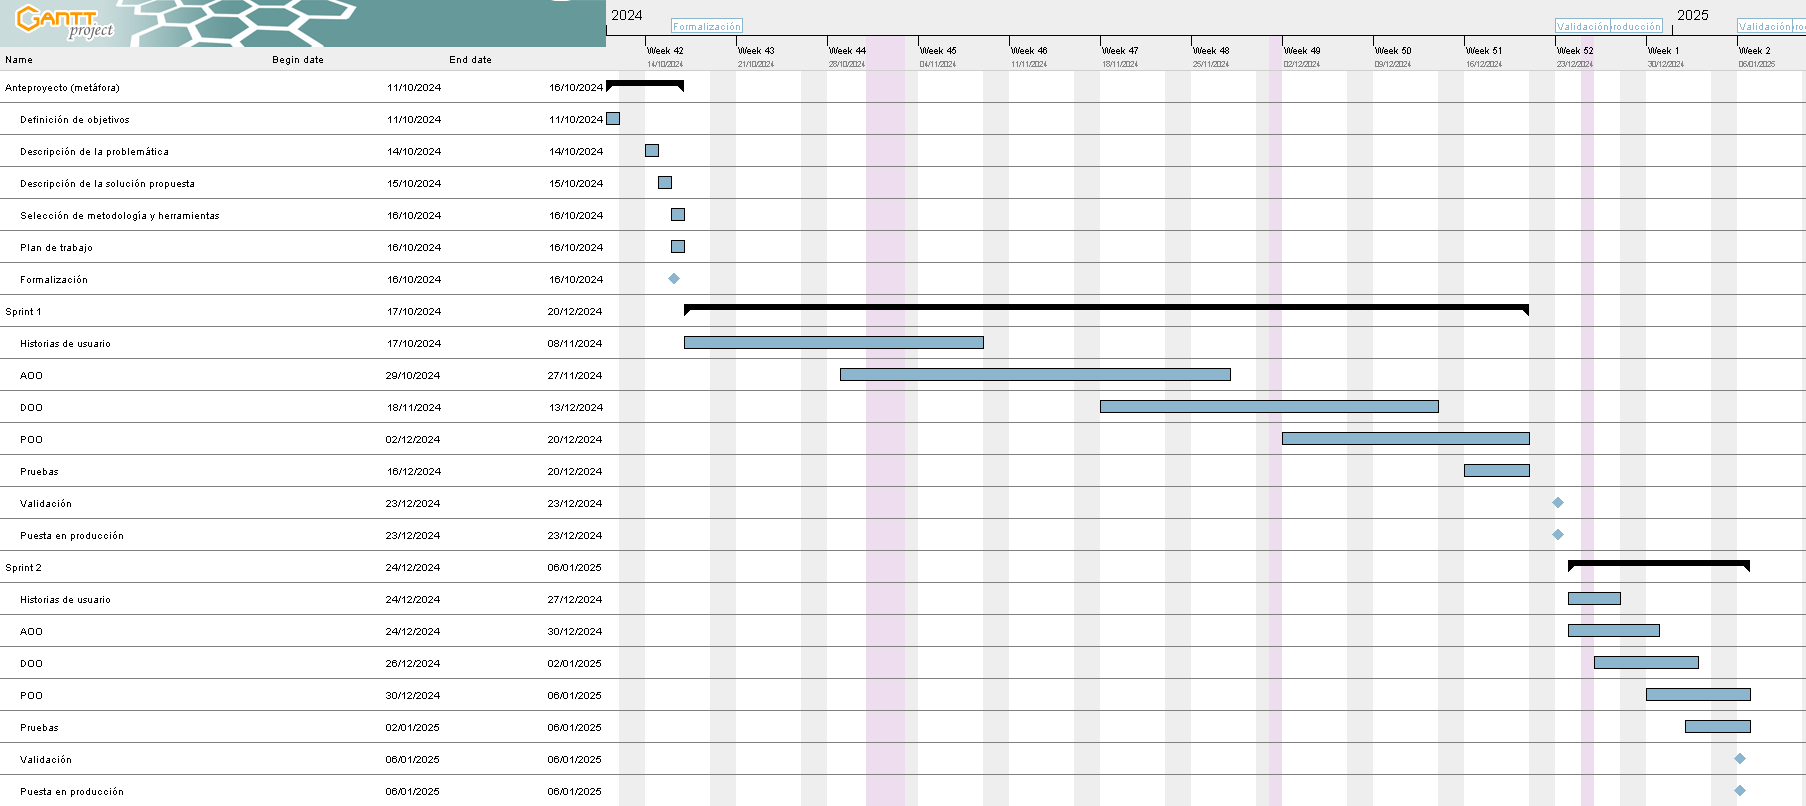
\includegraphics[width=\textwidth]{img/CartaGantt.png}
	\caption{Carta Gantt}
	\label{fig:CartaGantt}
\end{figure}
\clearpage
